% =====================================================================
% Relatório  Distribuição Normal (Curva de Gauss)
% Compilar com: pdflatex relatorio.tex (rodar duas vezes para o sumário)
% As figuras histograma_curva_normal.png e boxplot.png precisam estar
% na mesma pasta deste arquivo.
% =====================================================================
\documentclass[12pt,a4paper]{article}

% ---------------------------------------------------------------------
% Pacotes
% ---------------------------------------------------------------------
\usepackage[utf8]{inputenc}
\usepackage[T1]{fontenc}
\usepackage[brazil]{babel}
\usepackage{lmodern}
\usepackage{microtype}
\usepackage[a4paper,top=3cm,bottom=2cm,left=3cm,right=2cm,headheight=15pt]{geometry}
\usepackage{amsmath,amssymb}
\usepackage{icomma}          % vírgula como separador decimal no modo matemático
\usepackage{graphicx}
\usepackage{float}
\usepackage{booktabs}
\usepackage{array}
\usepackage{caption}
\usepackage{indentfirst}
\usepackage{enumitem}
\usepackage[dvipsnames]{xcolor}
\usepackage{listings}
\usepackage[most]{tcolorbox}
\usepackage{fancyhdr}
\usepackage{xurl}
\usepackage[hidelinks]{hyperref}

\setlength{\parskip}{0.4em}
\linespread{1.3}
\captionsetup{font=small,labelfont=bf}

% ---------------------------------------------------------------------
% Dados do trabalho (edite aqui)
% ---------------------------------------------------------------------
\newcommand{\instituicao}{Instituto Federal de Educação, Ciência e Tecnologia de São Paulo}
\newcommand{\campus}{Câmpus Itapetininga}
\newcommand{\curso}{Tecnologia em Sistemas para Internet}
\newcommand{\disciplina}{Probabilidade e Estatística Aplicada}
\newcommand{\professor}{Wilton Moreira Ferraz Junior}
\newcommand{\autor}{Mariana Alice Pires Leite (3043151)}
\newcommand{\titulo}{Distribuição Normal e Curva de Gauss}
\newcommand{\subtitulo}{Análise das notas de matemática da base \textit{Students Performance in Exams} com implementação em Python}

% ---------------------------------------------------------------------
% Caixas didáticas
% ---------------------------------------------------------------------
\newtcolorbox{exemplo}[1][]{
  enhanced, breakable,
  colback=blue!3, colframe=blue!50!black,
  fonttitle=\bfseries, title=Exemplo numérico #1,
  left=8pt, right=8pt, top=6pt, bottom=6pt
}
\newtcolorbox{destaque}[1]{
  enhanced, breakable,
  colback=orange!5, colframe=orange!70!black,
  fonttitle=\bfseries, title=#1,
  left=8pt, right=8pt, top=6pt, bottom=6pt
}

% ---------------------------------------------------------------------
% Código Python
% ---------------------------------------------------------------------
\lstset{
  language=Python,
  basicstyle=\ttfamily\small,
  keywordstyle=\color{blue!70!black}\bfseries,
  commentstyle=\color{gray}\itshape,
  stringstyle=\color{OliveGreen},
  numbers=left, numberstyle=\tiny\color{gray},
  frame=single, rulecolor=\color{gray!50},
  backgroundcolor=\color{gray!4},
  breaklines=true, showstringspaces=false,
  tabsize=4, columns=fullflexible, keepspaces=true,
  literate={á}{{\'a}}1 {à}{{\`a}}1 {ã}{{\~a}}1 {â}{{\^a}}1
           {é}{{\'e}}1 {ê}{{\^e}}1 {í}{{\'i}}1 {ó}{{\'o}}1
           {ô}{{\^o}}1 {õ}{{\~o}}1 {ú}{{\'u}}1 {ç}{{\c c}}1
           {μ}{{$\mu$}}1 {σ}{{$\sigma$}}1 {−}{{-}}1 {—}{{-}}1
}

% ---------------------------------------------------------------------
% Cabeçalho e rodapé
% ---------------------------------------------------------------------
\pagestyle{fancy}
\fancyhf{}
\fancyhead[L]{\small \titulo}
\fancyhead[R]{\small \thepage}
\renewcommand{\headrulewidth}{0.4pt}

\begin{document}

% =====================================================================
% CAPA
% =====================================================================
\begin{titlepage}
  \centering
  {\large \textbf{\instituicao}}\\[0.2cm]
  {\large \campus}\\[0.2cm]
  {\large \curso}\\[0.2cm]
  {\large \disciplina}\\
  \vfill
  {\LARGE \textbf{\titulo}}\\[0.6cm]
  {\large \subtitulo}\\
  \vfill
  {\large \autor}\\[1.2cm]
  {\large Prof. Dr. \professor}\\
  \vfill
  {\large Itapetininga}\\[0.2cm]
  {\large Novembro de 2026}
\end{titlepage}

\thispagestyle{empty}
\tableofcontents
\clearpage

% =====================================================================
\section{Introdução}
% =====================================================================

Este relatório apresenta o desenvolvimento de um programa em Python que carrega dados numéricos de um arquivo CSV, calcula medidas estatísticas, constrói gráficos e avalia se a variável analisada apresenta comportamento aproximadamente compatível com uma distribuição normal.

A base utilizada foi a \textit{Students Performance in Exams}, disponível no Kaggle no arquivo \texttt{StudentsPerformance.csv} (SPSCIENTIST, 2018). Ela possui 1.000 registros e oito colunas, com características dos estudantes e suas notas de matemática, leitura e escrita. A variável analisada foi a nota de matemática, armazenada na coluna \texttt{math score}, que contém valores inteiros entre 0 e 100.

Conforme as restrições da atividade, nenhum cálculo estatístico foi feito com bibliotecas prontas. O programa usa apenas os módulos \texttt{csv} e \texttt{math} para a leitura e os cálculos, e a biblioteca \texttt{matplotlib} (HUNTER, 2007) somente para os gráficos. Todos os resultados são obtidos a partir dos dados brutos do arquivo, sem valores inseridos manualmente.

As seções seguintes acompanham as partes da atividade. A Seção~\ref{sec:a} traz a pesquisa teórica, as Seções~\ref{sec:b} a \ref{sec:f} explicam o que o programa faz em cada etapa e os resultados obtidos, e a Seção~\ref{sec:g} apresenta a conclusão.

% =====================================================================
\section{Parte A: pesquisa teórica}\label{sec:a}
% =====================================================================

\subsection{Distribuição normal e Curva de Gauss}

A distribuição normal é uma distribuição de probabilidade \textbf{contínua}, ou seja, a variável pode assumir qualquer valor real. Ela é conhecida como Curva de Gauss em homenagem ao matemático Carl Friedrich Gauss, que a utilizou no estudo de erros de medição. Esse modelo é importante porque muitas variáveis influenciadas por vários fatores pequenos e independentes, como alturas, erros de medida e notas de provas, costumam se distribuir de forma próxima a ele (BUSSAB; MORETTIN, 2017).

O gráfico da distribuição normal tem formato de sino e apresenta as seguintes características.

\begin{itemize}[leftmargin=*]
  \item É \textbf{simétrico} em relação à média, com a metade esquerda espelhando a metade direita.
  \item A \textbf{média, a mediana e a moda são iguais} e ficam no centro da curva, onde está o ponto mais alto.
  \item As \textbf{caudas} se aproximam do eixo horizontal sem tocá-lo, o que indica que valores muito afastados do centro são raros, mas possíveis.
  \item A \textbf{área total} sob a curva é igual a 1, e a área entre dois pontos corresponde à probabilidade de a variável cair nesse intervalo.
\end{itemize}

A distribuição normal é determinada por dois parâmetros, a média $\mu$ e o desvio-padrão $\sigma$, e sua função densidade é

\begin{equation}\label{eq:densidade}
  f(x) = \frac{1}{\sigma\sqrt{2\pi}} \, e^{-\frac{(x-\mu)^2}{2\sigma^2}} .
\end{equation}

O termo $(x-\mu)^2$ no expoente negativo faz com que $f(x)$ diminua à medida que $x$ se afasta da média, formando as caudas. O fator $\frac{1}{\sigma\sqrt{2\pi}}$ garante que a área total seja 1. Essa foi a fórmula usada pelo programa para desenhar a curva teórica sobre o histograma.

\subsection{Função da média e do desvio-padrão}

A \textbf{média} $\mu$ define o \textbf{centro} da distribuição. Aumentar ou diminuir a média desloca a curva inteira para a direita ou para a esquerda, sem mudar seu formato.

O \textbf{desvio-padrão} $\sigma$ define a \textbf{dispersão}, ou seja, o quanto os valores se espalham em torno da média. Com $\sigma$ pequeno a curva fica alta e estreita, e com $\sigma$ grande ela fica baixa e larga.

Como os dados deste trabalho são uma amostra, a média é estimada por $\bar{x}$ e o desvio-padrão por $s$, o desvio-padrão amostral.

\subsection{Regra empírica 68--95--99,7}

Em dados normalmente distribuídos, a proporção de valores próximos da média é sempre a mesma, quaisquer que sejam $\mu$ e $\sigma$. Essa propriedade é chamada de regra empírica e afirma que aproximadamente

\begin{align*}
  68\%   &\text{ dos valores estão entre } \mu - \sigma  \text{ e } \mu + \sigma,\\
  95\%   &\text{ dos valores estão entre } \mu - 2\sigma \text{ e } \mu + 2\sigma,\\
  99{,}7\% &\text{ dos valores estão entre } \mu - 3\sigma \text{ e } \mu + 3\sigma.
\end{align*}

Assim, contar quantos dados caem em cada intervalo e comparar com esses percentuais é uma forma simples de avaliar se os dados se comportam de modo semelhante a uma distribuição normal.

\subsection{Escore padronizado \texorpdfstring{$z$}{z}}

O escore $z$ indica quantos desvios-padrão um valor está acima ou abaixo da média e é calculado por

\begin{equation}\label{eq:z}
  z = \frac{x - \mu}{\sigma} .
\end{equation}

Um valor $z=0$ é igual à média, um $z$ positivo está acima da média e um $z$ negativo está abaixo. Por exemplo, $z = -2$ indica um valor dois desvios-padrão abaixo da média. Pela regra empírica, valores com $|z|>3$ aparecem em apenas cerca de 0,3\% dos casos em dados normais, por isso são considerados \textbf{possíveis valores atípicos}.

% =====================================================================
\section{Parte B: leitura e organização dos dados}\label{sec:b}
% =====================================================================

\subsection{O que foi feito}

A função \texttt{carregar\_notas} abre o arquivo \texttt{StudentsPerformance.csv} com o módulo \texttt{csv} e usa a classe \texttt{csv.DictReader}. Essa classe lê a primeira linha como cabeçalho e transforma cada linha seguinte em um dicionário, de modo que a nota de cada estudante é acessada diretamente pelo nome da coluna, \texttt{registro["math score"]}.

Para cada registro, o programa faz três verificações antes de aceitar a nota.

\begin{enumerate}[leftmargin=*]
  \item Se o valor está \textbf{ausente}, isto é, vazio.
  \item Se o valor pode ser \textbf{convertido para inteiro} com \texttt{int()}. Caso não possa, é considerado inválido.
  \item Se a nota está dentro do \textbf{intervalo válido} de 0 a 100.
\end{enumerate}

As notas aprovadas são armazenadas em uma lista, e os problemas encontrados são guardados com o número da linha do arquivo, para que possam ser informados ao usuário. O trecho a seguir mostra o núcleo dessa leitura.

\noindent\begin{minipage}{\linewidth}
\begin{lstlisting}
leitor = csv.DictReader(arquivo)
for numero_linha, registro in enumerate(leitor, start=2):
    valor = registro.get("math score")
    if valor is None or valor.strip() == "":
        problemas.append((numero_linha, "valor ausente"))
        continue
    try:
        nota = int(valor.strip())
    except ValueError:
        problemas.append((numero_linha, "valor inválido"))
        continue
    if 0 <= nota <= 100:
        notas.append(nota)
\end{lstlisting}
\end{minipage}

\subsection{Resultado}

O programa leu \textbf{1.000 registros} e converteu todas as 1.000 notas de matemática para inteiros. \textbf{Não foram encontrados valores ausentes ou inválidos}, então todas as análises seguintes usam $n = 1000$ notas.

% =====================================================================
\section{Parte C: medidas estatísticas}\label{sec:c}
% =====================================================================

\subsection{O que foi feito}

Cada medida foi implementada em uma função própria, usando apenas laços, operações aritméticas e a função \texttt{math.sqrt} para a raiz quadrada. A Tabela~\ref{tab:formulas} resume como cada medida foi calculada.

\begin{table}[H]
  \centering
  \caption{Medidas calculadas e forma de cálculo.}
  \label{tab:formulas}
  \renewcommand{\arraystretch}{1.6}
  \begin{tabular}{>{\raggedright}p{4.2cm} p{10.5cm}}
    \toprule
    \textbf{Medida} & \textbf{Como foi calculada} \\
    \midrule
    Quantidade, menor e maior nota & Tamanho da lista e primeiro e último elementos da lista ordenada \\
    Amplitude total & $A = x_{\max} - x_{\min}$ \\
    Média aritmética & $\bar{x} = \dfrac{1}{n}\displaystyle\sum_{i=1}^{n} x_i$ \\
    Mediana & Valor central da lista ordenada. Como $n$ é par, é a média dos elementos nas posições $\frac{n}{2}$ e $\frac{n}{2}+1$ \\
    Moda ou modas & Dicionário com a frequência de cada nota, retornando todas as notas que empatam na maior frequência \\
    Variância amostral & $s^2 = \dfrac{\sum (x_i - \bar{x})^2}{n-1}$ \\
    Desvio-padrão amostral & $s = \sqrt{\dfrac{\sum (x_i - \bar{x})^2}{n-1}}$ \\
    Coeficiente de assimetria & $g = \dfrac{n}{(n-1)(n-2)} \displaystyle\sum \left(\dfrac{x_i - \bar{x}}{s}\right)^3$ \\
    \bottomrule
  \end{tabular}
\end{table}

Na variância e no desvio-padrão amostrais, divide-se por $n-1$ em vez de $n$. Essa correção compensa o fato de a média ter sido calculada com os próprios dados, o que tornaria a dispersão levemente subestimada.

O coeficiente de assimetria mede o quanto a distribuição se afasta da simetria. Como os desvios são elevados ao cubo, eles mantêm o sinal. Um valor negativo indica cauda mais longa à esquerda, um valor positivo indica cauda mais longa à direita, e um valor próximo de zero indica simetria. Foi adotada a interpretação de que $|g| < 0{,}1$ é aproximadamente simétrico, $0{,}1 \le |g| < 0{,}5$ é assimetria leve, $0{,}5 \le |g| < 1$ é moderada e $|g| \ge 1$ é forte.

\subsection{Resultado}

\begin{table}[H]
  \centering
  \caption{Medidas estatísticas das notas de matemática.}
  \label{tab:medidas}
  \begin{tabular}{l r}
    \toprule
    \textbf{Medida} & \textbf{Valor} \\
    \midrule
    Quantidade de dados ($n$)          & 1000 \\
    Menor nota                         & 0 \\
    Maior nota                         & 100 \\
    Amplitude total                    & 100 \\
    Média aritmética ($\bar{x}$)       & 66,0890 \\
    Mediana                            & 66 \\
    Moda                               & 65 (36 ocorrências) \\
    Variância amostral ($s^2$)         & 229,9190 \\
    Desvio-padrão amostral ($s$)       & 15,1631 \\
    Coeficiente de assimetria ($g$)    & $-0{,}2789$ \\
    \bottomrule
  \end{tabular}
\end{table}

\begin{exemplo}[(mediana e desvio-padrão)]
Como $n = 1000$ é par, a mediana é a média das notas nas posições 500 e 501 da lista ordenada. As duas valem 66, então a mediana é $\frac{66+66}{2} = 66$.

A variância obtida foi $s^2 = 229{,}9190$, expressa em pontos ao quadrado. Tirando a raiz, volta-se à unidade das notas, $s = \sqrt{229{,}9190} \approx 15{,}16$ pontos. Isso significa que, em geral, as notas se afastam cerca de 15 pontos da média.
\end{exemplo}

A média (66,09), a mediana (66) e a moda (65) ficaram muito próximas, como se espera em uma distribuição normal. O coeficiente de assimetria $g=-0{,}2789$ indica \textbf{leve assimetria negativa}, ou seja, a cauda das notas baixas é um pouco mais longa que a das notas altas.

% =====================================================================
\section{Parte D: regra 68--95--99,7}\label{sec:d}
% =====================================================================

\subsection{O que foi feito}

A função \texttt{regra\_empirica} calcula, para $k = 1$, 2 e 3, os limites $\bar{x} - k\,s$ e $\bar{x} + k\,s$. Em seguida, percorre a lista de notas contando quantas estão dentro de cada intervalo, e calcula o percentual dividindo essa contagem por $n$ e multiplicando por 100.

\subsection{Resultado}

\begin{table}[H]
  \centering
  \caption{Percentuais observados comparados à regra empírica.}
  \label{tab:regra}
  \begin{tabular}{c c c c c c}
    \toprule
    \textbf{Intervalo} & \textbf{Limites} & \textbf{Qtd.} & \textbf{Observado} & \textbf{Esperado} & \textbf{Diferença} \\
    \midrule
    $\bar{x} \pm 1s$ & [50,93; 81,25]  & 696 & 69,60\% & 68\%   & $+1{,}60$ p.p. \\
    $\bar{x} \pm 2s$ & [35,76; 96,42]  & 954 & 95,40\% & 95\%   & $+0{,}40$ p.p. \\
    $\bar{x} \pm 3s$ & [20,60; 111,58] & 996 & 99,60\% & 99,7\% & $-0{,}10$ p.p. \\
    \bottomrule
  \end{tabular}
\end{table}

\begin{exemplo}[(primeiro intervalo)]
Com $\bar{x} = 66{,}0890$ e $s = 15{,}1631$, os limites de $\bar{x} \pm 1s$ são $66{,}0890 - 15{,}1631 = 50{,}93$ e $66{,}0890 + 15{,}1631 = 81{,}25$. Como as notas são inteiras, esse intervalo vai da nota 51 à nota 81. Na base há 696 notas nessa faixa, o que corresponde a $\frac{696}{1000} \times 100 = 69{,}60\%$.
\end{exemplo}

Os três percentuais ficaram muito próximos dos teóricos, com diferença máxima de 1,6 ponto percentual. O intervalo de um desvio-padrão ficou um pouco acima do esperado, o que mostra uma concentração ligeiramente maior de notas em torno da média. Também é interessante notar que o limite superior do terceiro intervalo, 111,58, passa da nota máxima possível, que é 100.

% =====================================================================
\section{Parte E: escores padronizados}\label{sec:e}
% =====================================================================

\subsection{O que foi feito}

A função \texttt{escore\_z} aplica a Equação~\eqref{eq:z} usando $\bar{x}$ e $s$ no lugar de $\mu$ e $\sigma$. Ela foi aplicada à menor nota, à maior nota e às notas 50, 75 e 90. Cada resultado foi classificado como possível valor atípico quando $|z|>3$. Além disso, o programa percorreu toda a base para listar todas as notas que atendem a esse critério.

\subsection{Resultado}

\begin{table}[H]
  \centering
  \caption{Escores $z$ das notas solicitadas.}
  \label{tab:z}
  \begin{tabular}{l c r l}
    \toprule
    \textbf{Caso} & \textbf{Nota} & \textbf{Escore $z$} & \textbf{Classificação} \\
    \midrule
    Menor nota & 0   & $-4{,}3585$ & Possível valor atípico \\
    Maior nota & 100 & $2{,}2364$  & Dentro do esperado \\
    Nota 50    & 50  & $-1{,}0611$ & Dentro do esperado \\
    Nota 75    & 75  & $0{,}5877$  & Dentro do esperado \\
    Nota 90    & 90  & $1{,}5769$  & Dentro do esperado \\
    \bottomrule
  \end{tabular}
\end{table}

\begin{exemplo}[(nota 75)]
\[
  z = \frac{75 - 66{,}0890}{15{,}1631} = \frac{8{,}9110}{15{,}1631} \approx 0{,}5877 .
\]
O valor positivo mostra que a nota 75 está acima da média, a uma distância de pouco mais de meio desvio-padrão.
\end{exemplo}

Apenas a menor nota, 0, foi classificada como possível valor atípico entre os casos pedidos, pois está mais de quatro desvios-padrão abaixo da média. Ao analisar toda a base, o programa encontrou \textbf{quatro notas com $|z|>3$}, que são 0, 8, 18 e 19. Elas representam 0,4\% dos dados e estão todas na cauda inferior, o que é coerente com a leve assimetria negativa.

% =====================================================================
\section{Parte F: representação gráfica}\label{sec:f}
% =====================================================================

\subsection{O que foi feito}

A função \texttt{gerar\_histograma} usa o \texttt{matplotlib} para construir o histograma das notas com classes de largura 5, de 0 a 100. Foi usada a opção \texttt{density=True}, que transforma a altura das barras em densidade e faz a área total do histograma valer 1. Isso permite comparar o histograma diretamente com a curva normal, cuja área também vale 1.

A curva normal teórica foi desenhada calculando a Equação~\eqref{eq:densidade} em 1.001 pontos entre 0 e 100, com a média e o desvio-padrão obtidos na Parte C. Foram adicionadas uma linha vertical na média e duas linhas tracejadas em $\bar{x} - s$ e $\bar{x} + s$. O resultado foi salvo como \texttt{histograma\_curva\_normal.png}. Também foi gerado o gráfico de caixa opcional, salvo como \texttt{boxplot.png}.

\subsection{Resultado}

\begin{figure}[H]
  \centering
  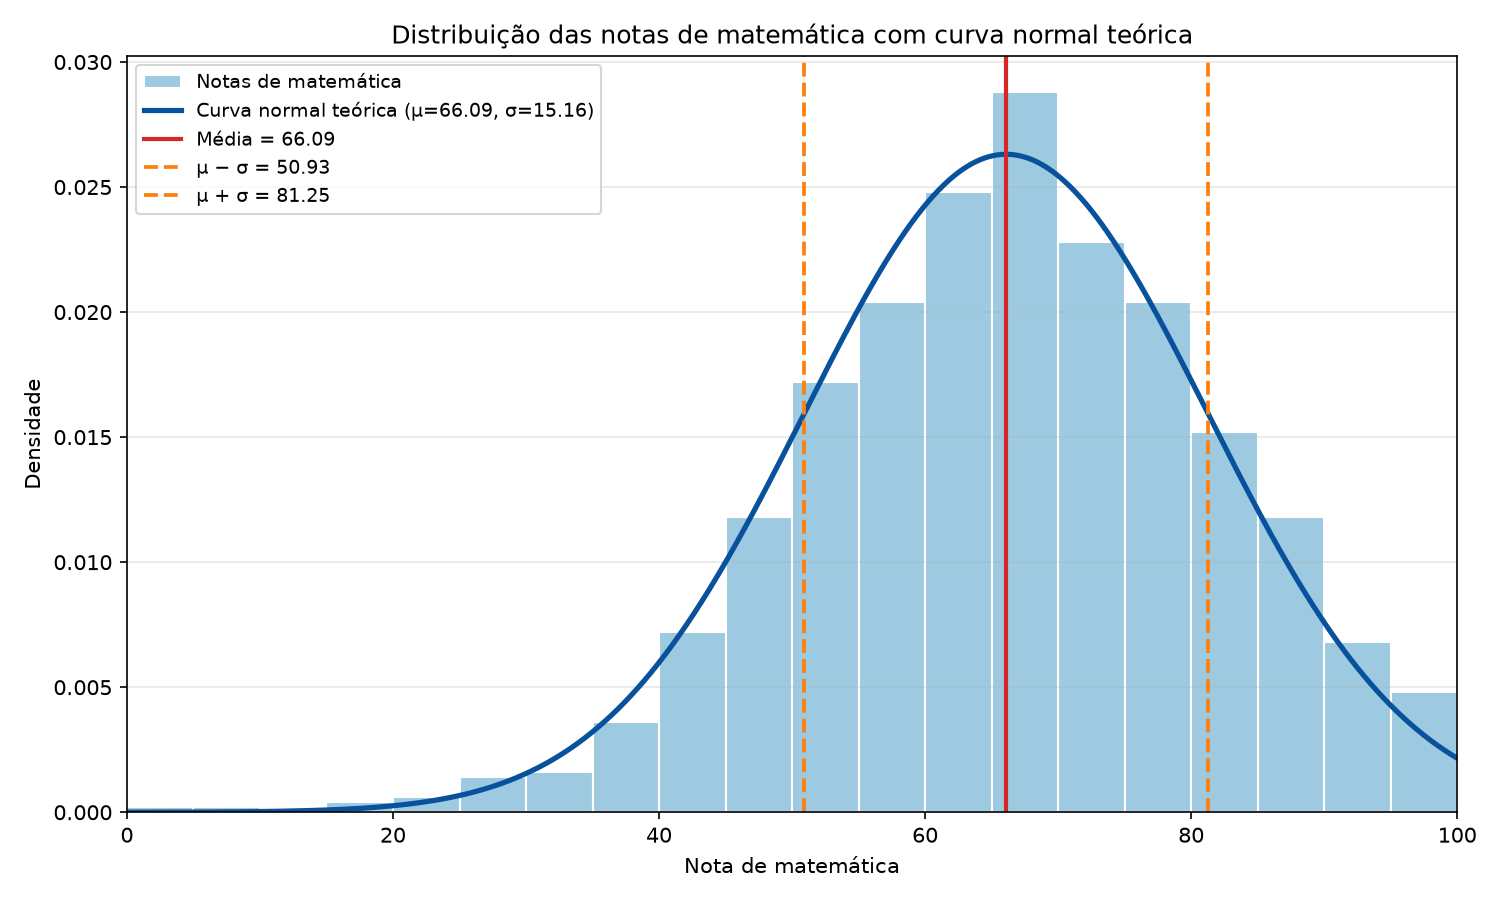
\includegraphics[width=\textwidth]{histograma_curva_normal.png}
  \caption{Histograma das notas de matemática com a curva normal teórica. A linha vermelha marca a média e as tracejadas marcam $\bar{x} \pm s$.}
  \label{fig:histograma}
\end{figure}

O histograma tem formato de sino bem definido, com as barras mais altas perto da média e diminuindo em direção às extremidades. A curva teórica acompanha de perto o contorno das barras. As principais diferenças são a classe de 65 a 70, que fica acima da curva, e a cauda esquerda, que se estende até a nota 0, enquanto a direita termina no limite de 100.

\begin{figure}[H]
  \centering
  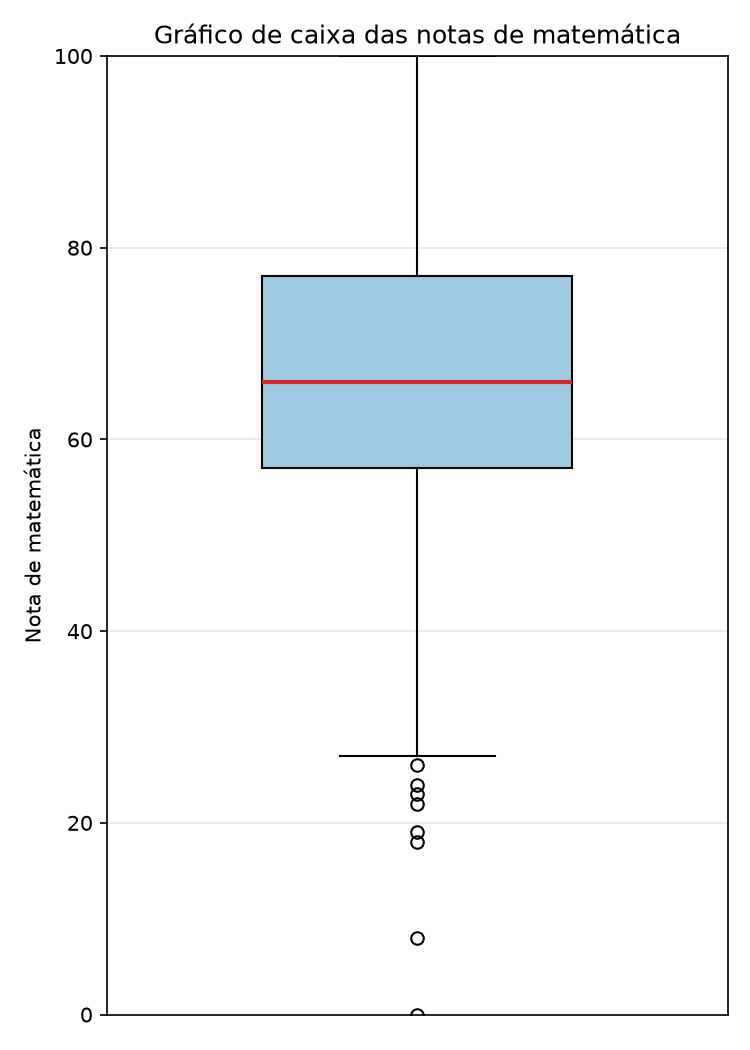
\includegraphics[width=0.42\textwidth]{boxplot.png}
  \caption{Gráfico de caixa das notas de matemática.}
  \label{fig:boxplot}
\end{figure}

No gráfico de caixa, a mediana está praticamente no centro da caixa, indicando que a parte central dos dados é quase simétrica. Os pontos isolados aparecem só abaixo da caixa, confirmando que os valores extremos estão entre as notas baixas.

% =====================================================================
\section{Parte G: conclusão}\label{sec:g}
% =====================================================================

\paragraph{O histograma apresenta aproximadamente o formato de sino?}
Sim. O histograma tem um pico central próximo da média e frequências que diminuem gradualmente nas duas direções, e a curva normal teórica acompanha bem o contorno das barras.

\paragraph{Média e mediana apresentam valores próximos?}
Sim. A média foi 66,089 e a mediana foi 66, uma diferença de apenas 0,089 ponto. A moda, 65, também está muito próxima, o que indica uma distribuição quase simétrica.

\paragraph{Os percentuais observados são próximos da regra 68--95--99,7?}
Sim. Os valores observados foram 69,60\%, 95,40\% e 99,60\%, contra 68\%, 95\% e 99,7\% esperados. A maior diferença foi de 1,6 ponto percentual, no intervalo de um desvio-padrão.

\paragraph{A distribuição apresenta assimetria?}
Sim, mas leve. O coeficiente de assimetria foi $-0{,}2789$, indicando assimetria negativa leve, causada por algumas notas muito baixas que alongam a cauda esquerda.

\paragraph{Existem valores atípicos?}
Sim. Quatro notas apresentaram $|z|>3$, que são 0, 8, 18 e 19. O critério indica apenas possíveis valores atípicos. Essas notas não são necessariamente erros, pois podem representar estudantes que realmente tiveram desempenho muito baixo, e por isso foram mantidas na análise.

\paragraph{É adequado afirmar que os dados seguem perfeitamente uma distribuição normal?}
Não. A distribuição normal é contínua, simétrica e admite qualquer valor real, enquanto as notas são inteiras, limitadas entre 0 e 100 e apresentam leve assimetria negativa. O próprio limite de 111,58 do intervalo de três desvios-padrão mostra que o modelo admite valores impossíveis para uma nota. Além disso, as técnicas usadas neste trabalho são descritivas e visuais, e não testes formais de normalidade.

\paragraph{Qual seria uma conclusão mais cuidadosa sobre a distribuição das notas?}
As notas de matemática apresentam \textbf{comportamento aproximadamente normal}. O histograma tem formato de sino, as medidas de tendência central são praticamente iguais e os percentuais da regra empírica estão muito próximos dos teóricos. Por outro lado, há uma leve assimetria negativa e alguns valores atípicos na cauda inferior. Portanto, a distribuição normal é um modelo adequado para descrever de forma geral o desempenho dos estudantes, desde que seja entendida como uma aproximação, e não como uma descrição exata dos dados.

% =====================================================================
\section*{Referências}
\addcontentsline{toc}{section}{Referências}

\begin{itemize}[leftmargin=0pt,label={},itemsep=0.8em]
  \setlength{\baselineskip}{1em}
  \item BUSSAB, W. O.; MORETTIN, P. A. \textbf{Estatística básica}. 9. ed. São Paulo: Saraiva, 2017.
  \item HUNTER, J. D. Matplotlib: a 2D graphics environment. \textbf{Computing in Science \& Engineering}, v. 9, n. 3, p. 90-95, 2007. DOI: \url{https://doi.org/10.1109/MCSE.2007.55}.
  \item SPSCIENTIST. \textbf{Students performance in exams}. [\textit{S. l.}]: Kaggle, 2018. Disponível em: \url{https://www.kaggle.com/datasets/spscientist/students-performance-in-exams}. Acesso em: 10 nov. 2026.
\end{itemize}

\end{document}
